\chapter{Rundgang durch den Open Stage-Modus}

Die Benutzung des ctGameStudio beginnt mit dem Login mit seinem persönlichen Benutzeraccount (Abb.
\ref{login}). Daraufhin wird das Spiel geladen, und das Hauptmenü angezeigt (Abb.  \ref{main-menu}).
Hier kann sich der Spieler entscheiden, den Storymodus oder den neuen Open Stage-Modus namens
\enquote{RoboStrategy} zu spielen. Hinter dem RoboStrategy-Menüpunkt verbirgt sich ein weiteres Menü
(Abb. \ref{openstage-menu}) zur Wahl zwischen Training oder Turnieren.

\section{Training}

Das Training (Abb. \ref{training}) zeigt die aus dem Storymodus bekannte Benutzeroberfläche mit
Strategieeditor auf der linken Seite und Arena auf der rechten Seite. In der Werkzeugleiste des
Editors befindet sich das die Oberfläche für das Strategiemanagment. Über das Dropdown-Menü kann auf
andere bereits gespeicherte Strategien gewechselt werden. Mit den weiteren Buttons kann die aktuelle
Strategie gespeichert, kopiert und gelöscht werden. Nebenher befinden sich die bereits im Storymodus
verfügbaren Buttons für den Zugang zu einer Dokumentation der verfügbaren Programmierblöcke und zur
Expansion des Strategieeditors (vgl. Abb. \ref{training-expanded}).

Die Arena wurde um Statusleiste erweitert, die die Lebensanzeigen der Roboter und eine Uhr zur
Anzeige der Ausführungszeit enthält. Die Werkzeugleiste unter der Arena enthält die Bedienelemente
zur Steuerung der Ausführung. Über das
Gegnerstrategie-Dropdown kann die Gegnerstrategie festgelegt werden. Hier stehen die drei
vorgefertigten und selbst angelegte Strategien zur Auswahl.

Im Editor wird eine Strategie durch die Anordnung von Blöcken generiert. Über den grünen
Ausführen-Button wird der Kampf gestartet. Abb. \ref{training-run} zeigt das Training während der
Ausführung eines Kampfes. Der Pause-Button wird die aktuelle Ausführung angehalten, während
Zurücksetzen-Button die Ausführung beendet und die Lebenspunkte der Roboter zurück setzt. Da zur
Evaluation seiner Strategie gewünscht sein mag, bei einer erneuten Ausführung den gleichen
Ausgangspunkt zu haben, zum Beispiel, wenn ein Fehler in der Strategie nur auftritt, wenn der
Roboter sich an einer bestimmten Position auf der Spielfläche befindet, kann über die
\enquote{Startpositionen beibehalten}-Option die Randomisierung der Startpositionen ausgeschaltet
werden.


\begin{figure}
  \centering
  \label{login}
  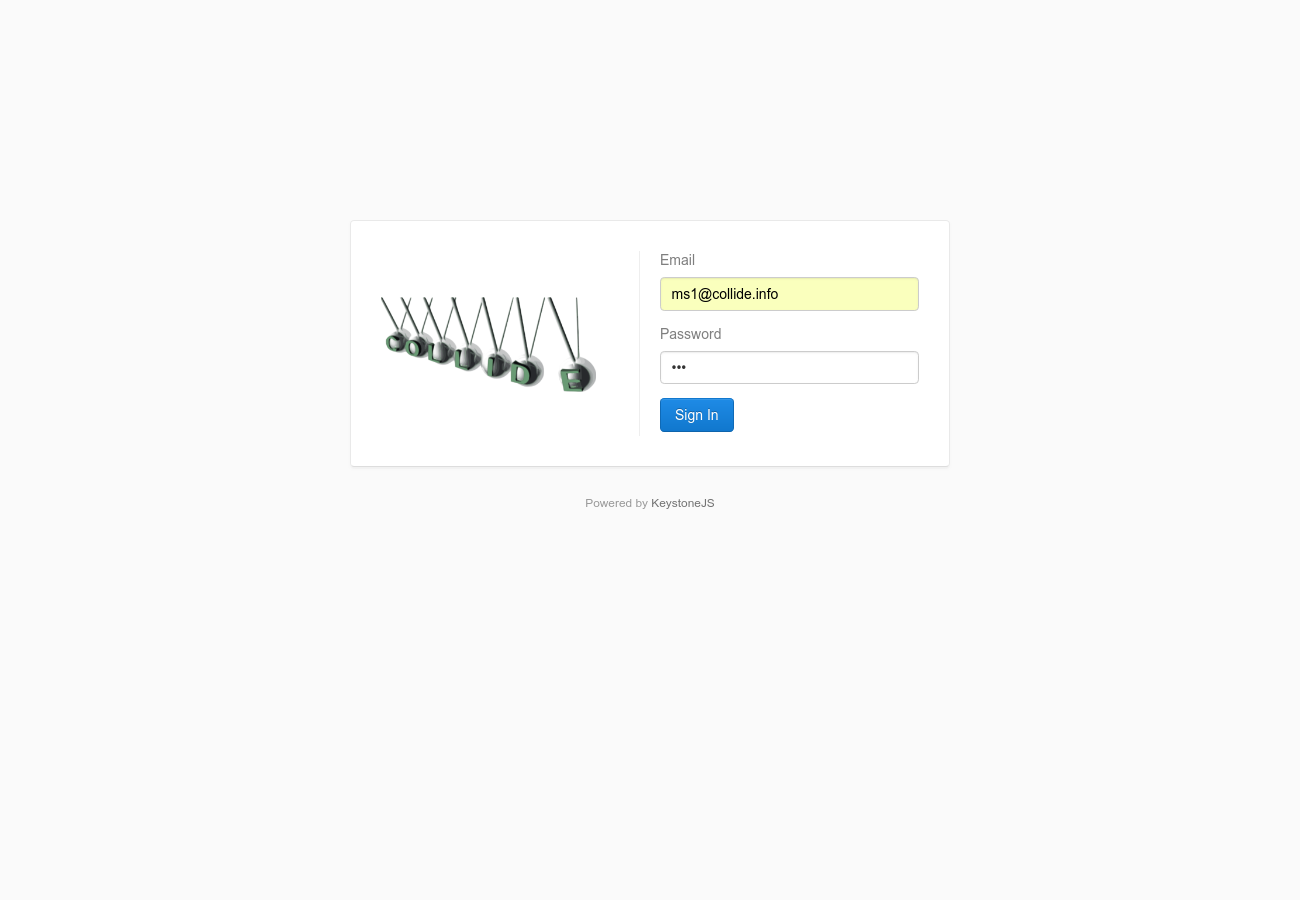
\includegraphics[width=15cm, height=10cm, keepaspectratio]{figures/1-login.png}
  \caption{Der Login-Dialog}
\end{figure}

\begin{figure}
  \centering
  \label{main-menu}
  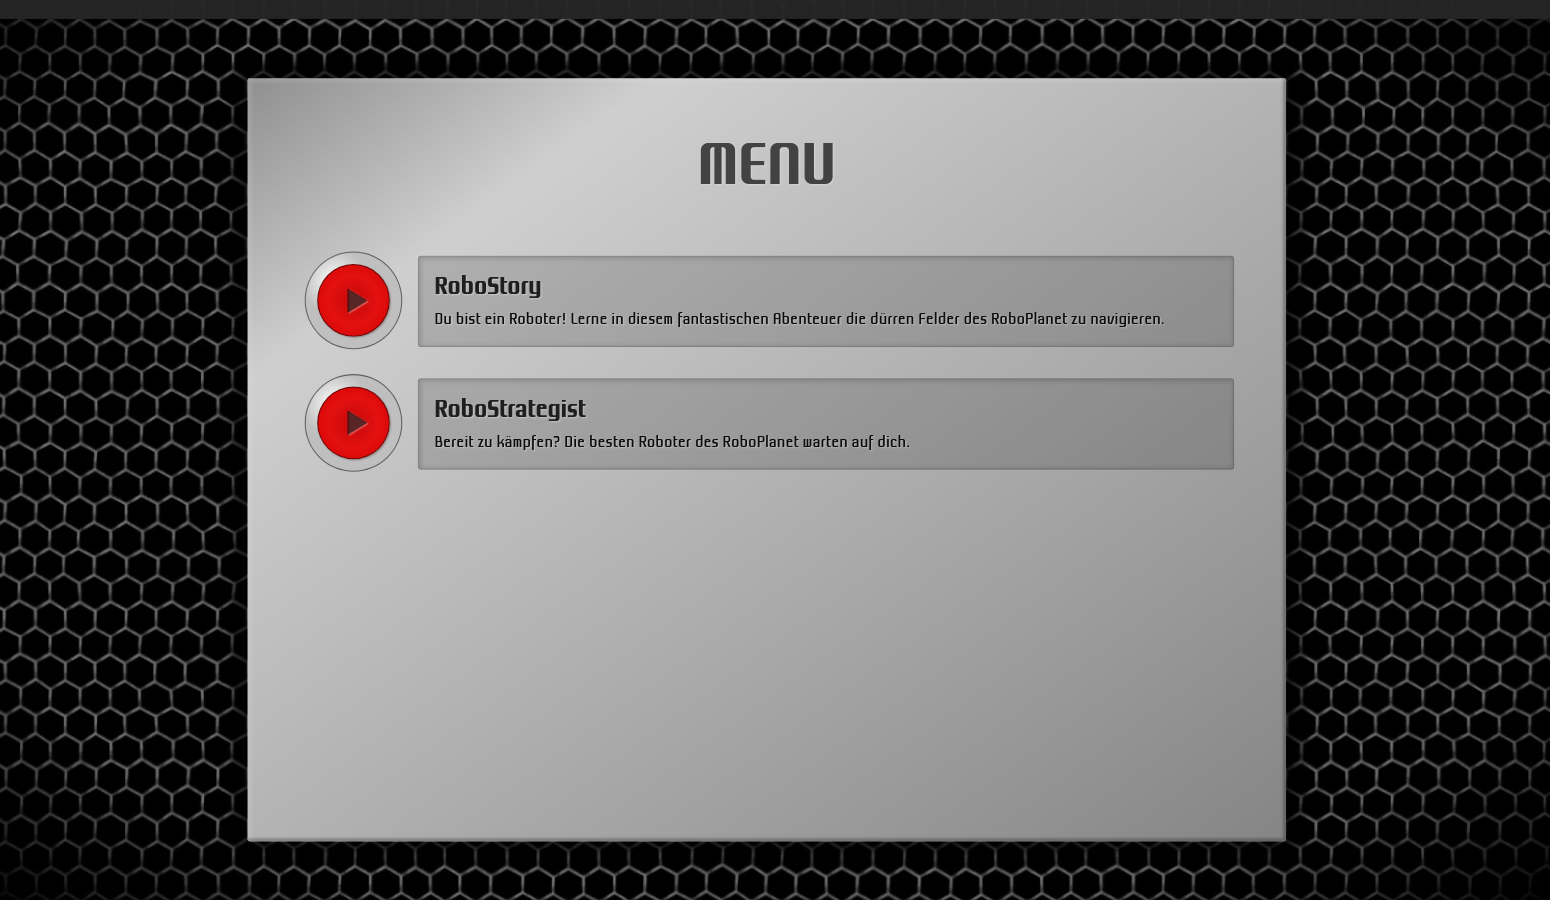
\includegraphics[width=15cm, keepaspectratio]{figures/2-main-menu.png}
  \caption{Das Hauptmenü}
\end{figure}

\begin{figure}
  \centering
  \label{openstage-menu}
  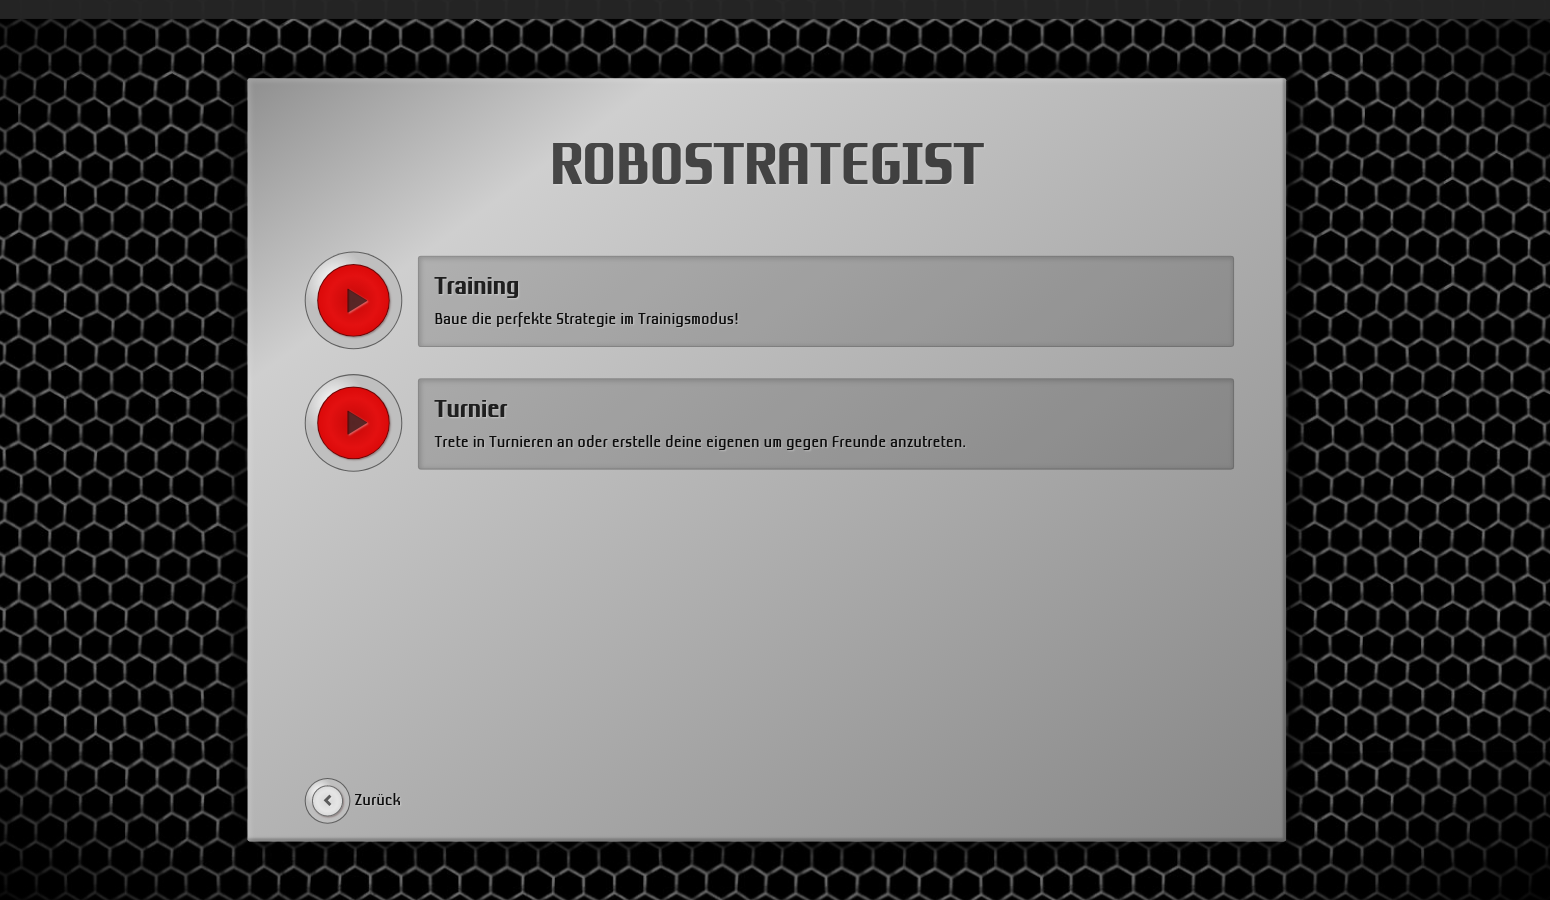
\includegraphics[width=15cm, keepaspectratio]{figures/3-robostrategist-menu.png}
  \caption{Menü des Open Stage-Modus}
\end{figure}

\begin{figure}
  \centering
  \label{training}
  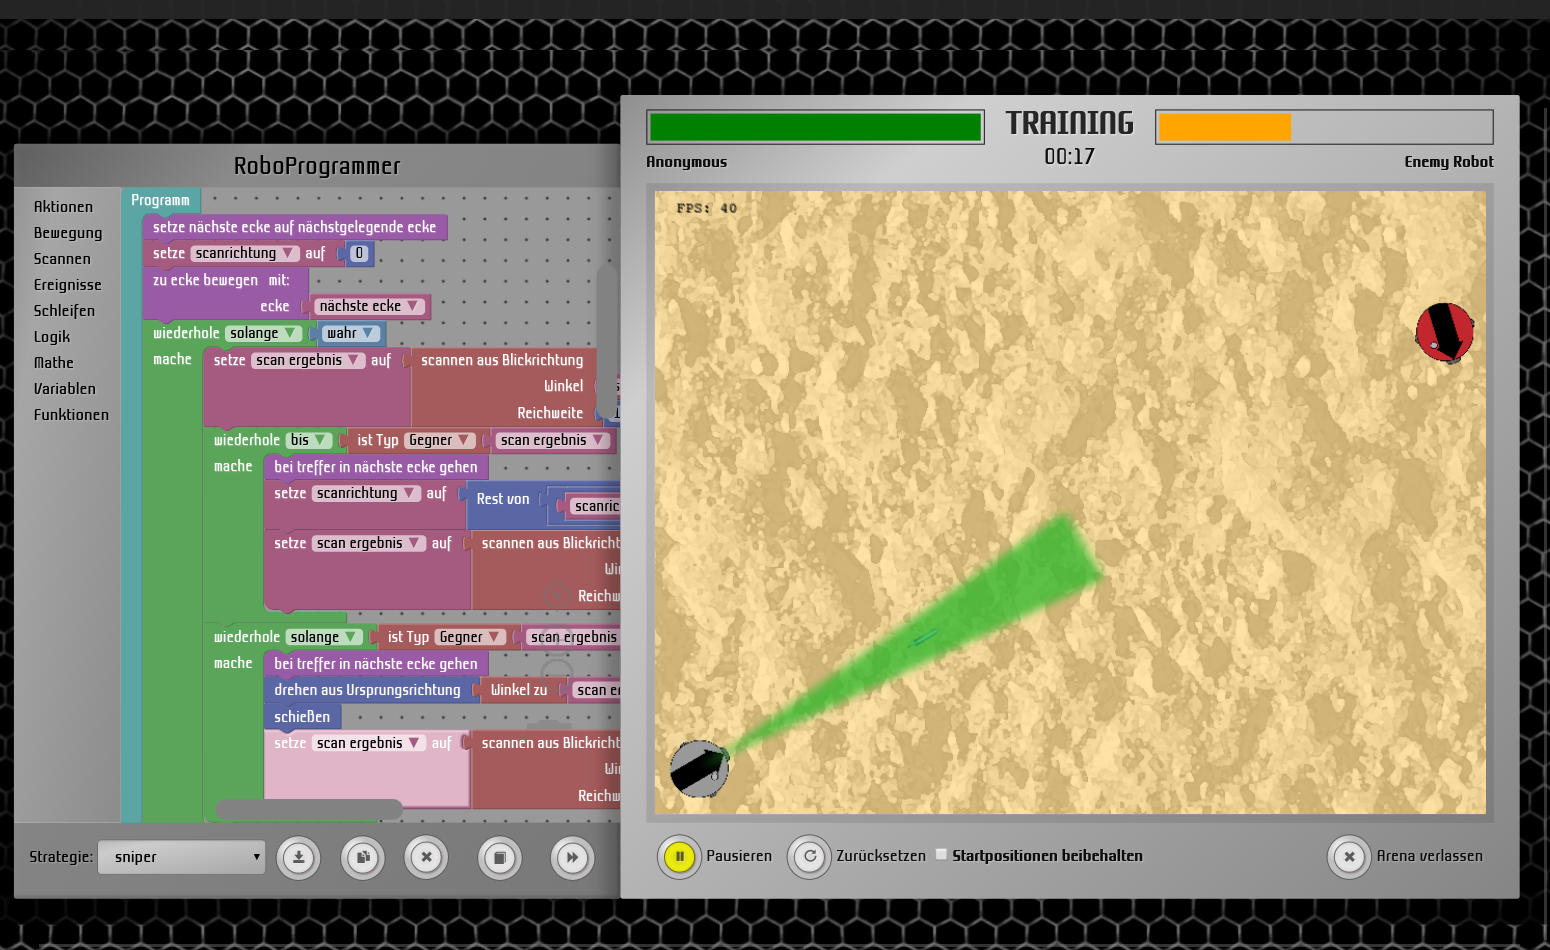
\includegraphics[width=15cm, keepaspectratio]{figures/3-training.png}
  \caption{Die Benutzeroberfläche des Trainings nach erstem Öffnen}
\end{figure}

\begin{figure}
  \centering
  \label{training-expanded}
  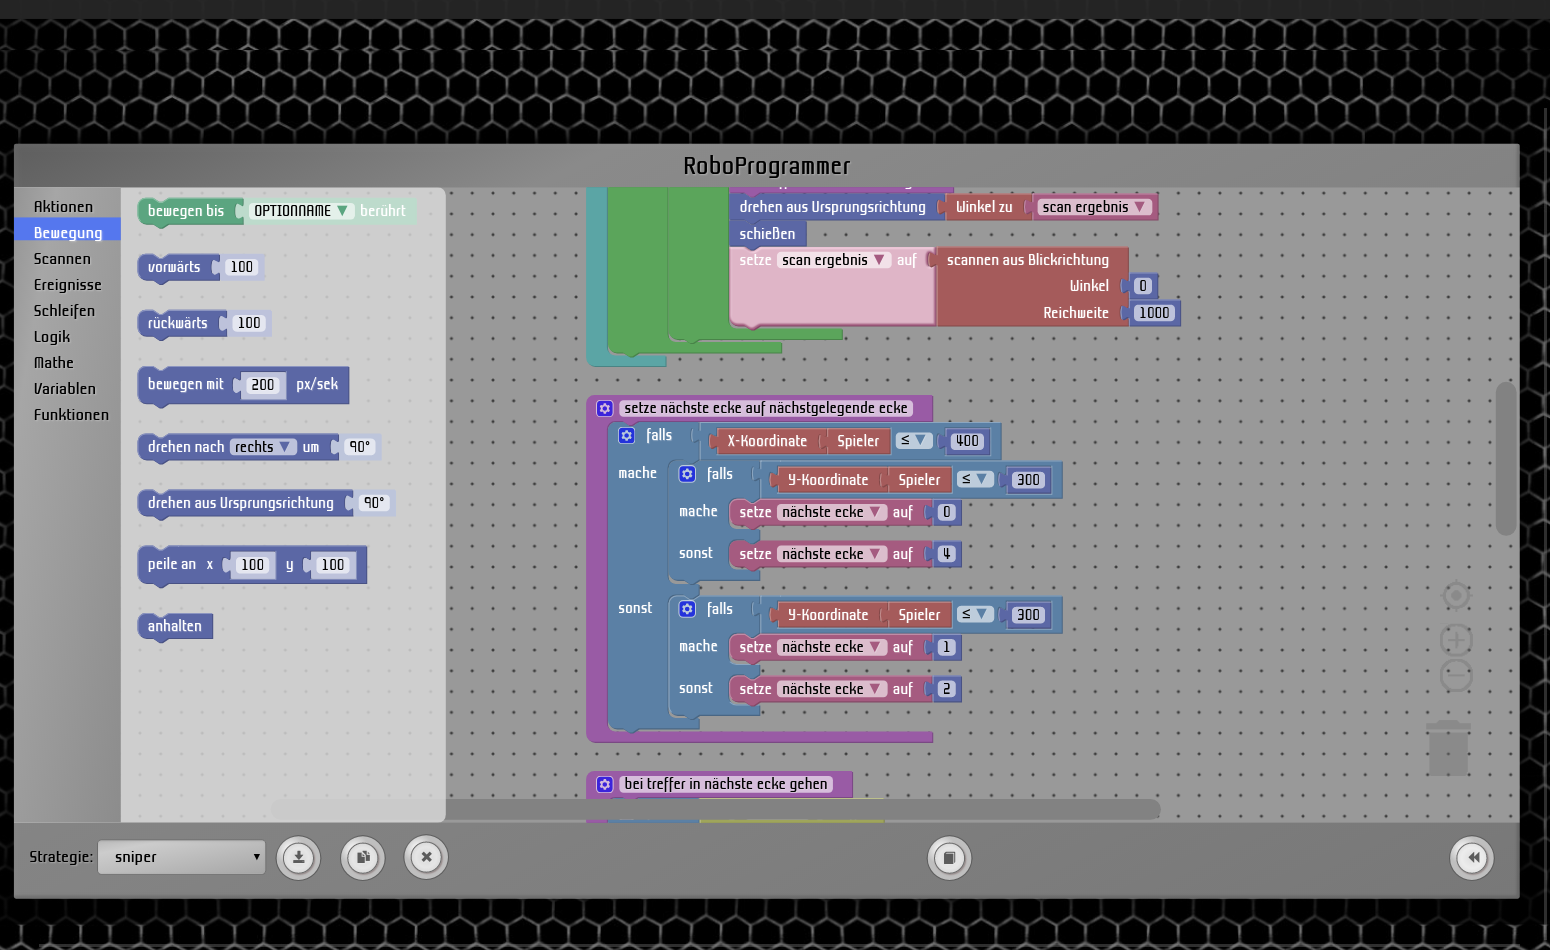
\includegraphics[width=15cm, keepaspectratio]{figures/4-training-expanded.png}
  \caption{Der Strategieeditor im expandiertem Zustand}
\end{figure}

\begin{figure}
  \centering
  \label{training-run}
  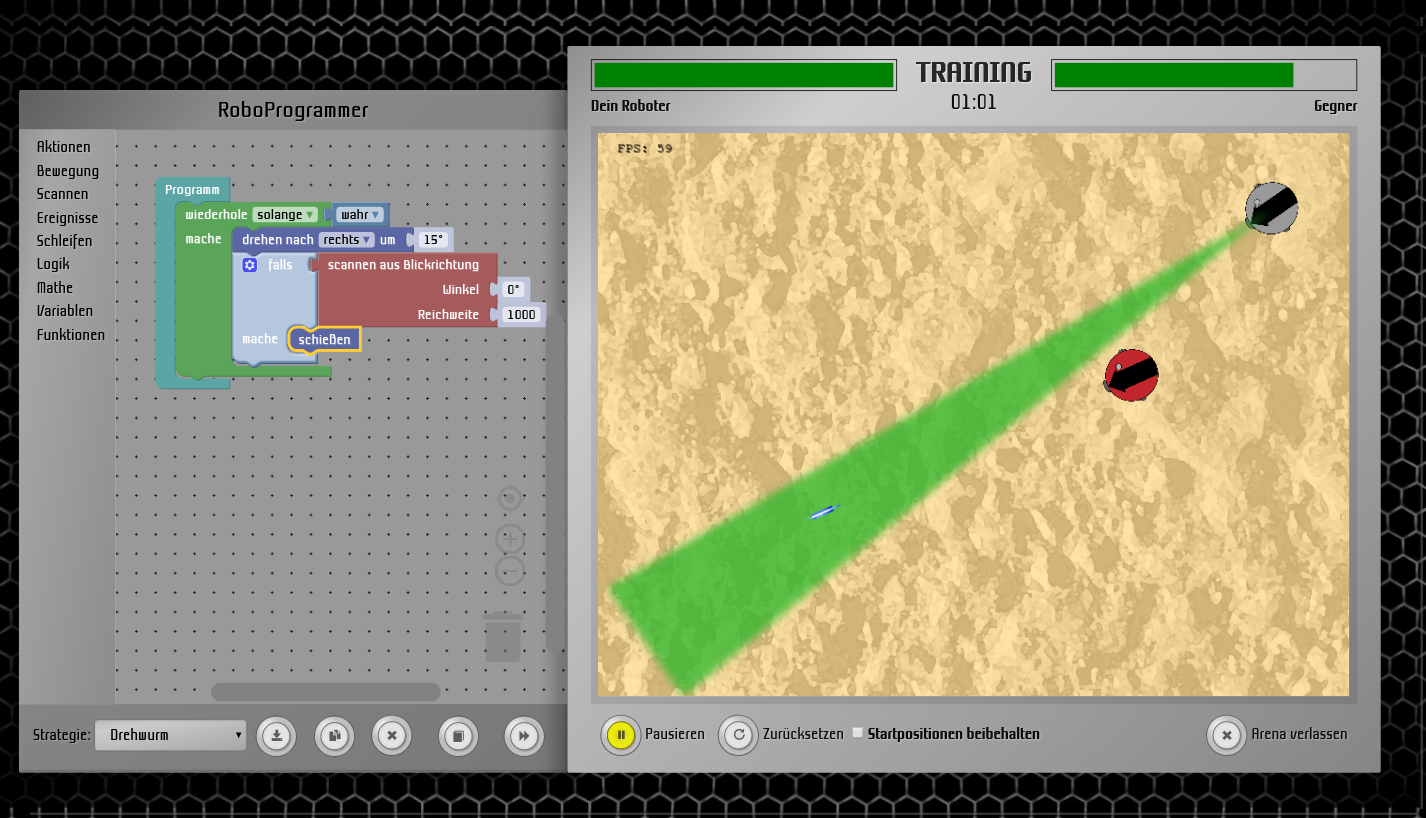
\includegraphics[width=15cm, keepaspectratio]{figures/3-training-run.png}
  \caption{Die Benutzeroberfläche des Trainings während der Ausführung einer Strategie}
\end{figure}


\section{Turniere}

Über das Turniermenü (Abb. \ref{tournament-menu}) werden die Turnier-bezogenen Dialoge erreicht.
Zunächst muss ein Turnier erstellt werden (Abb. \ref{create-tournament}). Dabei können
Turniersystem und Kampfoptionen nach Vorlieben festgelegt werden. Nach der Erstellung des Turniers
wird der Zugangscode generiert (Abb. \ref{create-tournament-code}). Dieser kann nun über Kanäle
außerhalb des Spiels an potentielle Teilnehmer weiter gegeben werden. Ein Spieler kann diesen Code
dann im Dialog zur Teilnahme am Turnier (Abb. \ref{participate-tournament}) angeben, um sich am
Turnier einzuschreiben. Dabei gibt er die Strategie an, mit der er kämpfen möchte. Um das Turnier zu
verfolgen, muss der 

Die Turnierliste enthält Übersicht über alle vom Spieler erstellten Turniere (Abb.
\ref{tournament-list}). In der Turnierlobby (Abb. \ref{tournament-lobby}) kann genau eingesehen
werden, wer am Turnier teilnimmt, und das Turnier gestartet werden. Daraufhin wird die Übersicht der
Turnierdurchführung geöffnet.

Falls der Verlauf des Turniers mit anderen geteilt werden soll, sollte
die Ansicht über Screen Sharing oder eine Projektion mit Interessierten geteilt werden. Abb.
\ref{tournament-execution-start} zeigt die Übersicht eines Jeder-gegen-Jeden-Turniers mit drei
Teilnehmern. Die Liste von Kämpfen gibt eine Vorausschau über den Verlauf des Turnieres, während
die Rangliste das Resultat des Turniers zeigt. Der Turnierersteller kann nun das erste Match
starten. Daraufhin wird die Übersicht durch die Ansicht der Arena ersetzt (Abb.
\ref{tournament-execution-match}), und der Kampf zwischen den Strategien, die von den Teilnehmern
eingereicht wurden, ausgeführt. Über den \enquote{Match unterbrechen...}-Button wird der Kampf
pausiert. Über ein Pausemenü (nicht abgebildet) kann der Kampf dann fortgefahren oder beendet werden.

Nach Ende des Kampfes erscheint wieder die Übersicht des Turniers. Abb.
\ref{tournament-execution-mid} zeigt ein Durchgang, bei denen Spielerin Franzi Hansel den ersten
Kampf gewonnen hat. Abb. \ref{tournament-execution-end}. zeigt die Turnierübersicht nach Ende des
letzten Kampfes.

Abb.
\ref{tournament-execution-ko-start} und \ref{tournament-execution-ko-end} zeigen die
Übersicht eines Turniers im KO-System in Form des Turnierbaums.

\begin{figure}
  \centering
  \label{tournament-menu}
  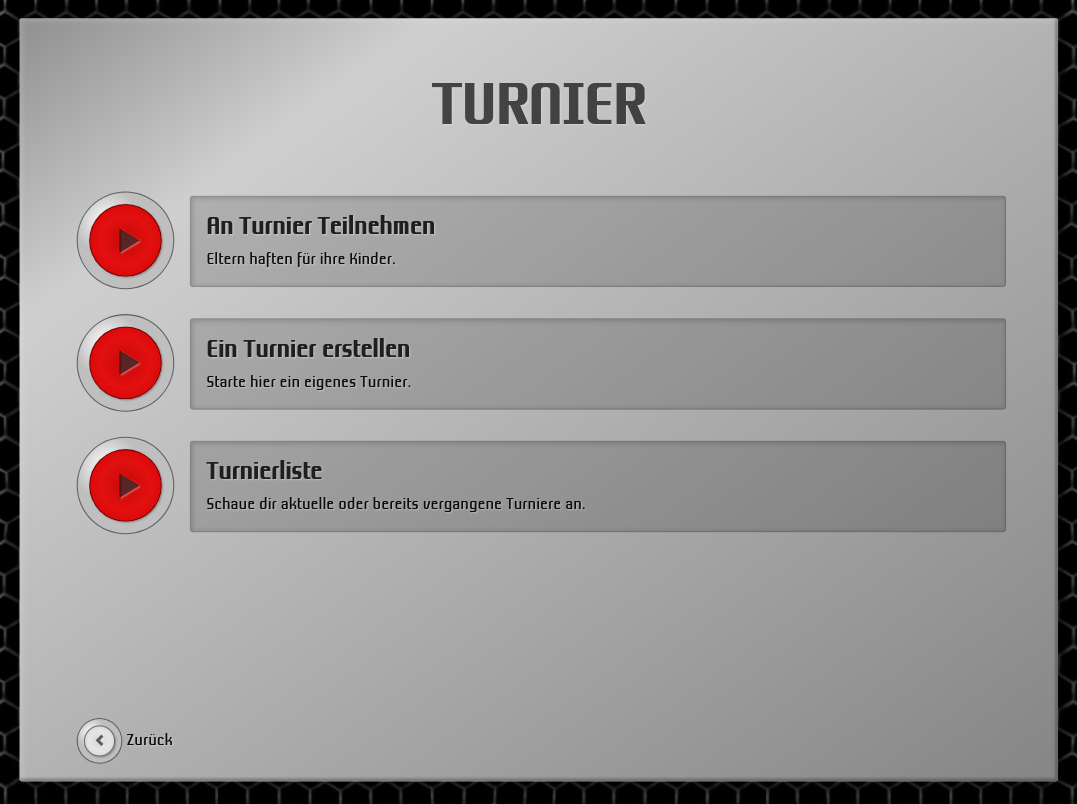
\includegraphics[width=15cm, keepaspectratio]{figures/5-turniermenu.png}
  \caption{Das Turniermenü}
\end{figure}

\begin{figure}
  \centering
  \label{create-tournament}
  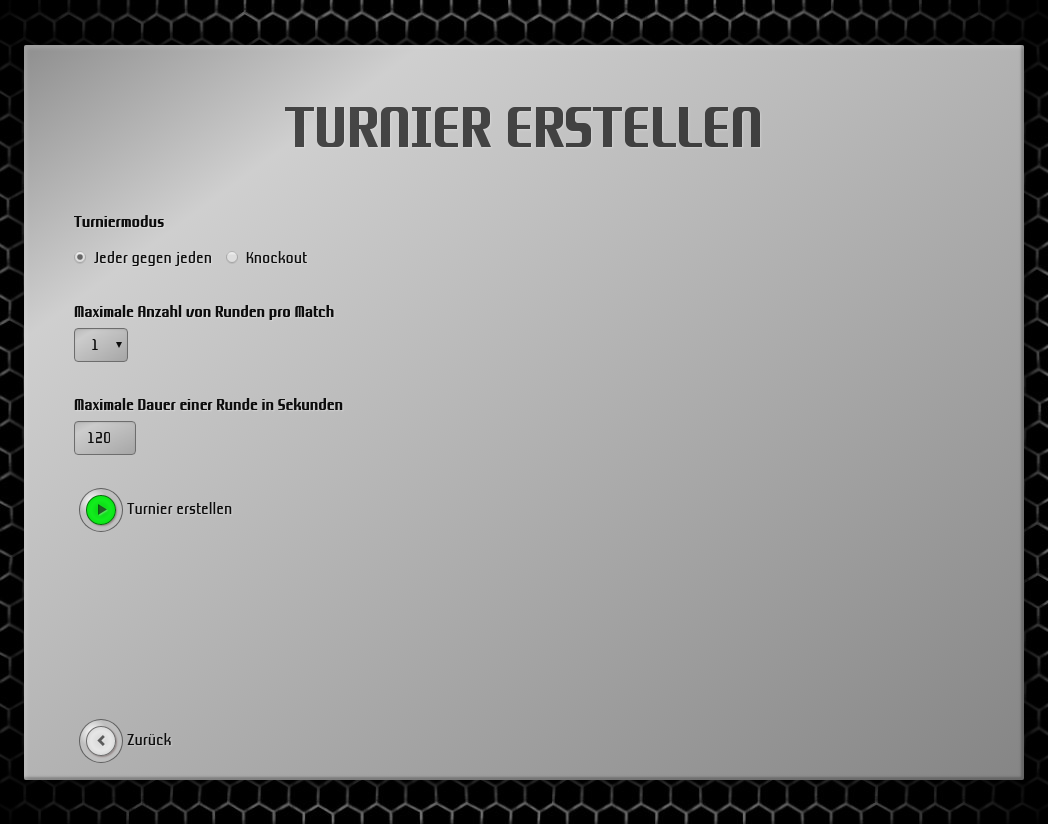
\includegraphics[width=15cm, keepaspectratio]{figures/6-turnier-erstellen-jgj.png}
  \caption{Der Dialog zum Erstellen des Turniers}
\end{figure}

\begin{figure}
  \centering
  \label{create-tournment-code}
  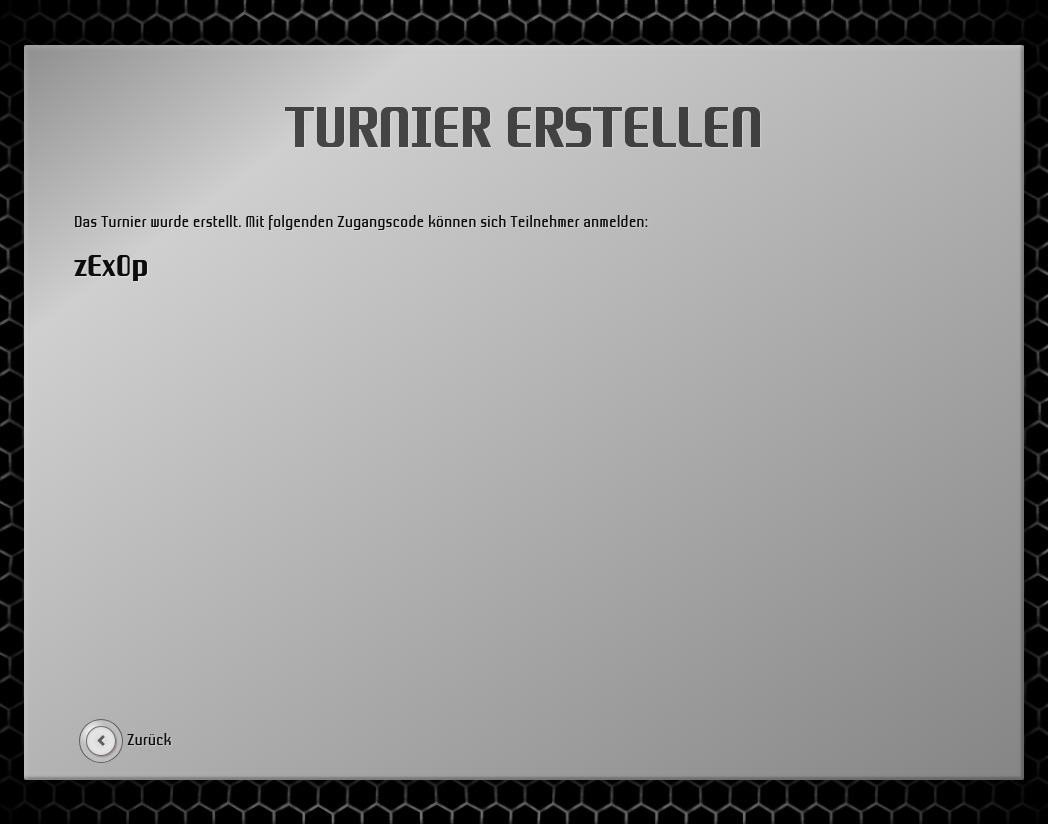
\includegraphics[width=15cm, keepaspectratio]{figures/7-turnier-erstellen-code.png}
  \caption{Der Zugangscode zum Turnier nach Erstellung des Turniers}
\end{figure}

\begin{figure}
  \centering
  \label{participate-tournament}
  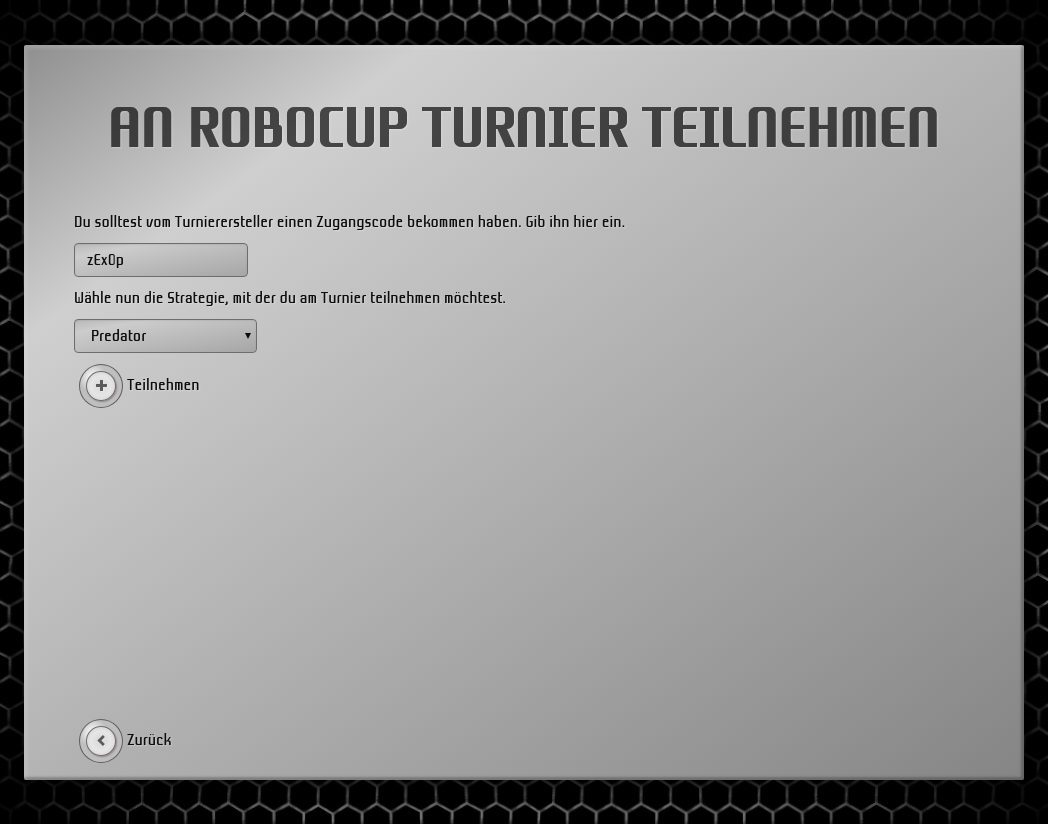
\includegraphics[width=15cm, keepaspectratio]{figures/9-turnierteilnahme.png}
  \caption{Der Dialog zur Teilnahme am Turnier}
\end{figure}

\begin{figure}
  \centering
  \label{tournament-lobby}
  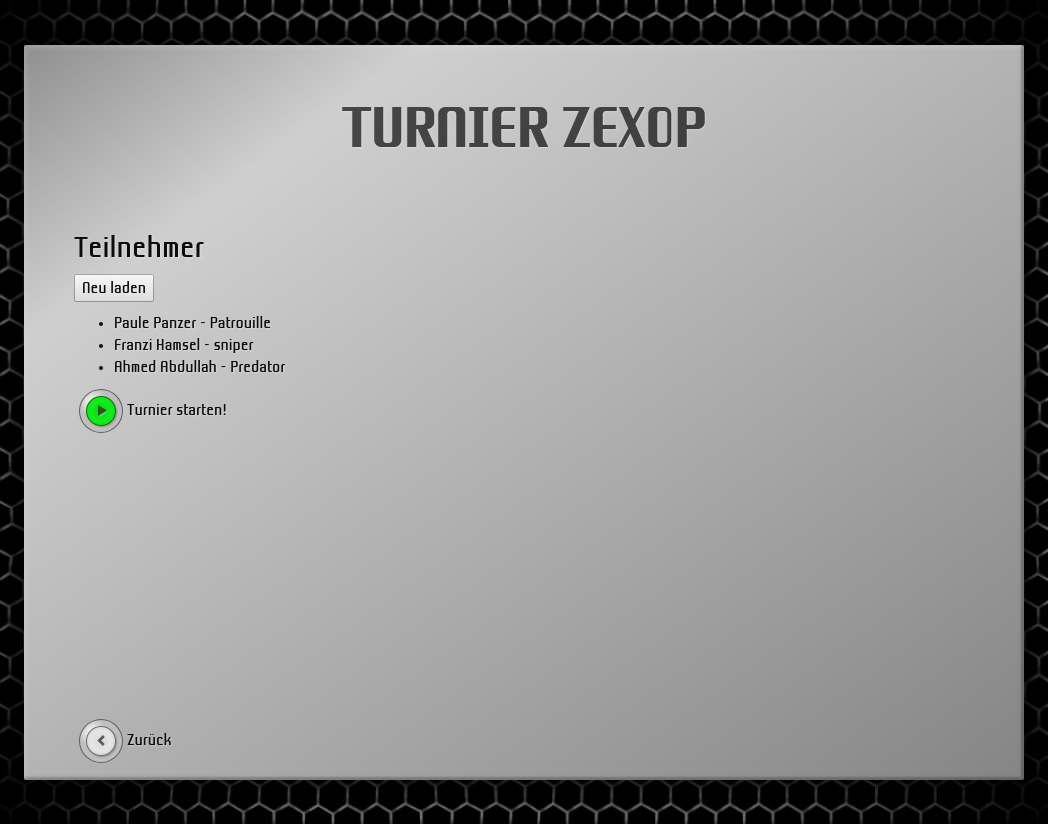
\includegraphics[width=15cm, keepaspectratio]{figures/10-turnierlobby.png}
  \caption{Die Turnierlobby}
\end{figure}

\begin{figure}
  \centering
  \label{tournament-list}
  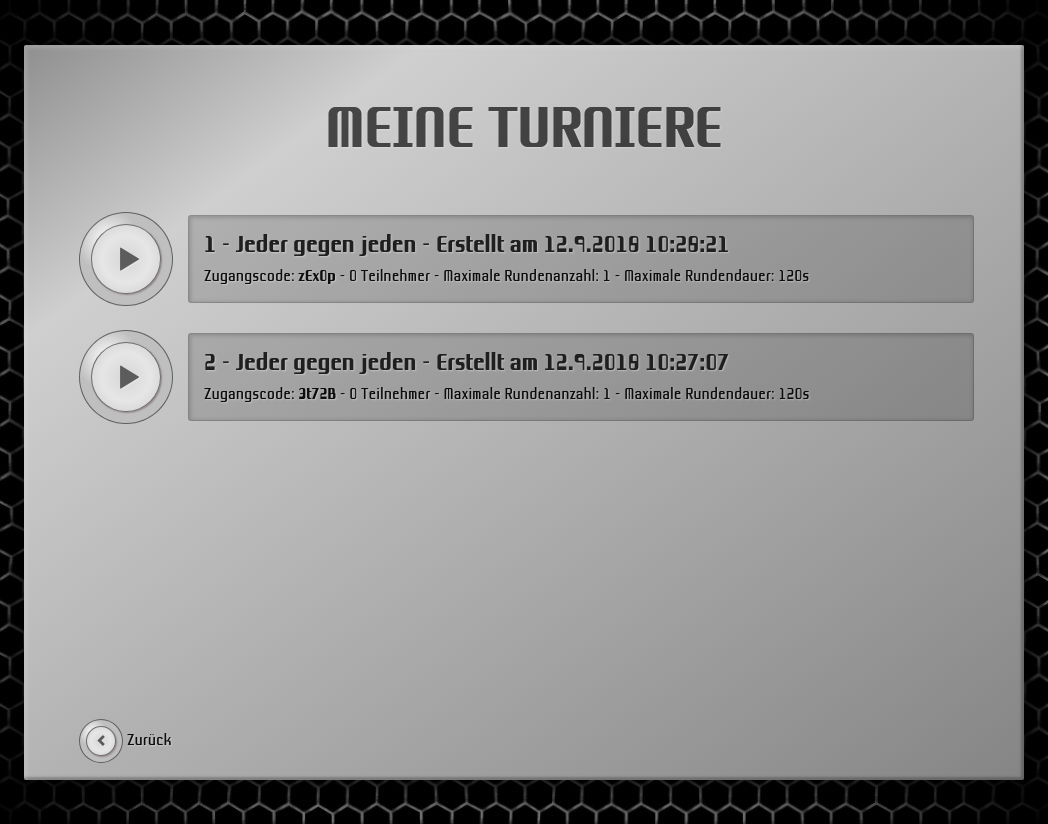
\includegraphics[width=15cm, keepaspectratio]{figures/8-turnierliste.png}
  \caption{Die Turnierliste}
\end{figure}

\begin{figure}
  \centering
  \label{tournament-execution-start}
  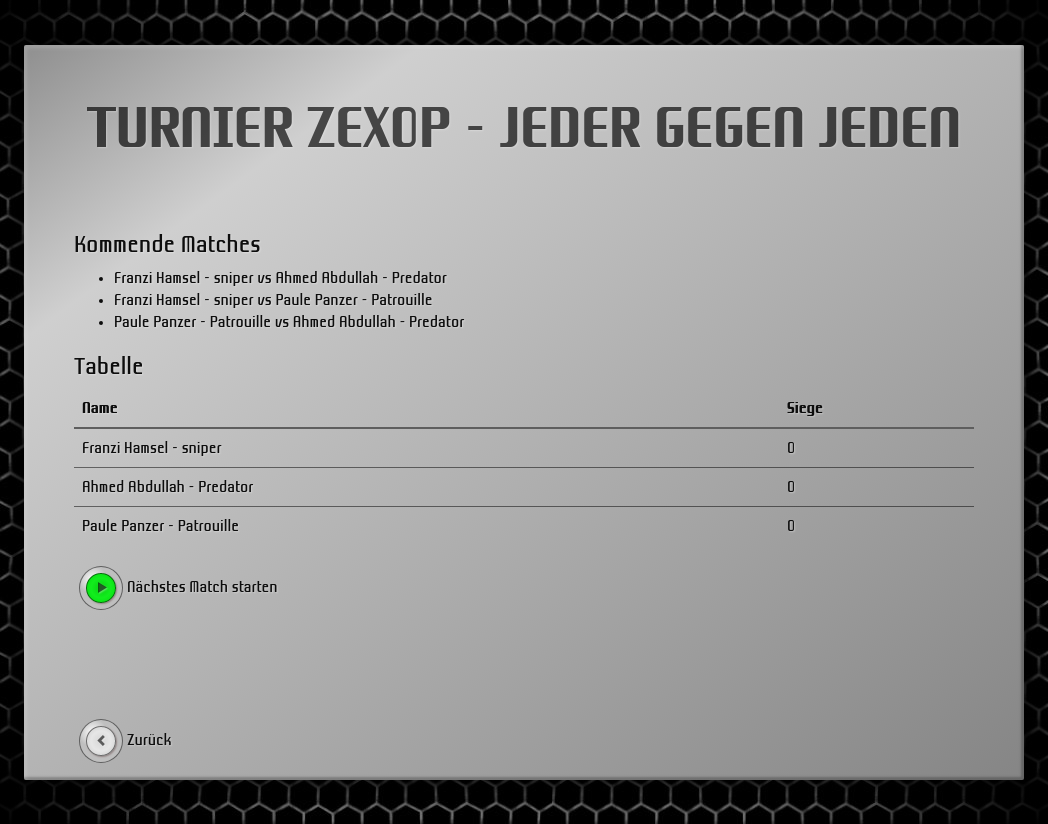
\includegraphics[width=15cm, keepaspectratio]{figures/11-turnierdurchfuehrung-start.png}
  \caption{Die Übersicht zur Turnierdurchführung im Jeder-gegen-Jeden-System zu Beginn eines Turniers}
\end{figure}

\begin{figure}
  \centering
  \label{tournament-execution-match}
  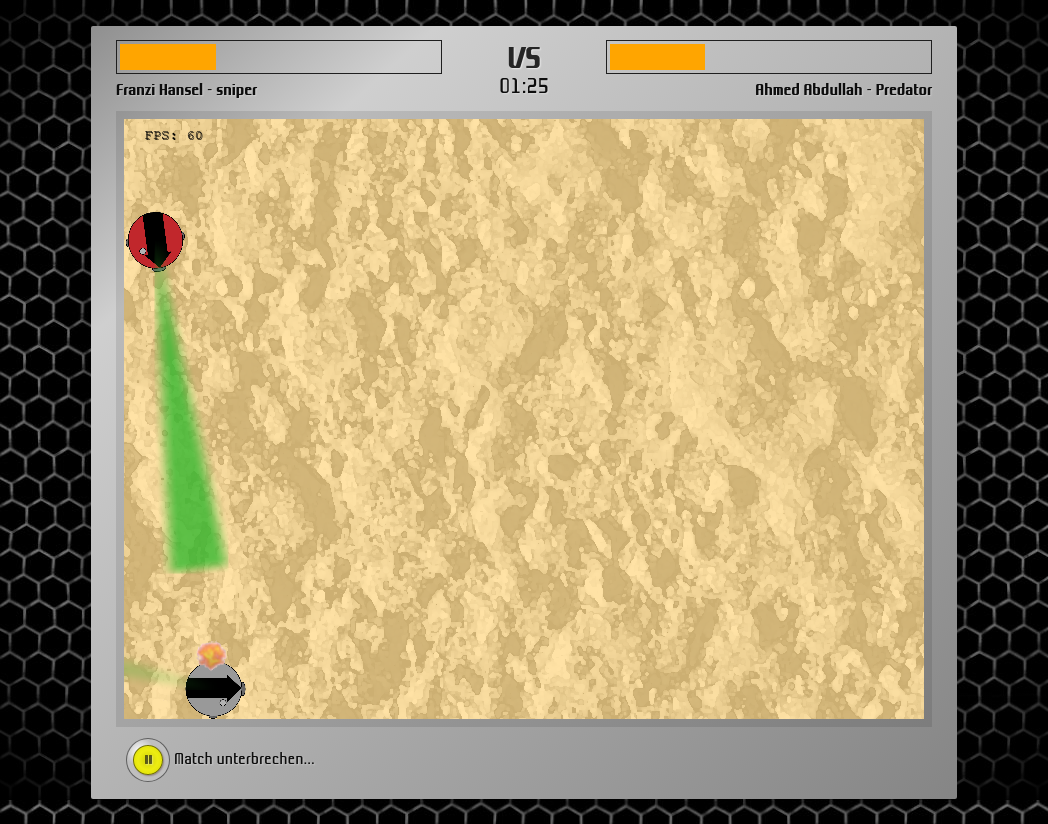
\includegraphics[width=15cm, keepaspectratio]{figures/14-turnierdurchfuehrung-kampf.png}
  \caption{Die Ansicht eines Turnierkampfes}
\end{figure}

\begin{figure}
  \centering
  \label{tournament-execution-mid}
  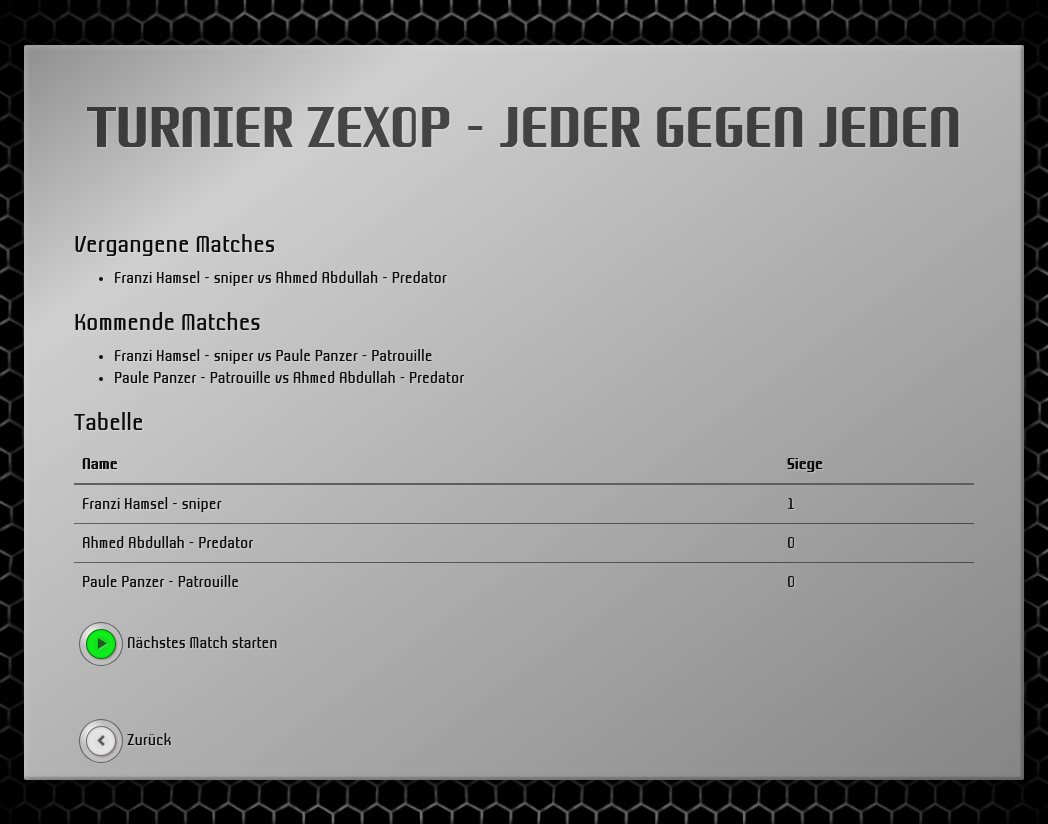
\includegraphics[width=15cm, keepaspectratio]{figures/13-turnierdurchfuehrung-mitte.png}
  \caption{Die Übersicht zur Turnierdurchführung im Jeder-gegen-Jeden-System nachdem ein Kampf durchgeführt wurde}
\end{figure}

\begin{figure}
  \centering
  \label{tournament-execution-end}
  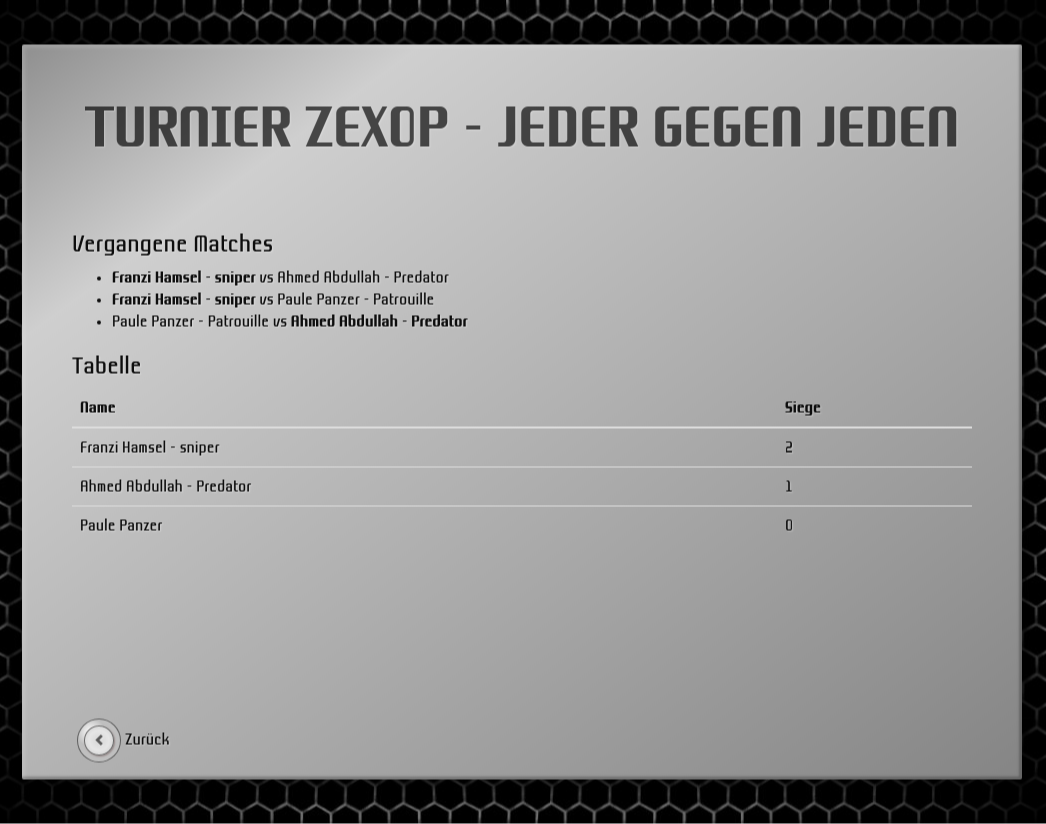
\includegraphics[width=15cm, keepaspectratio]{figures/15-turnierdurchfuehrung-ende.png}
  \caption{Die Übersicht zur Turnierdurchführung im Jeder-gegen-Jeden-System nach Ende des letzten Kampfes}
\end{figure}

\begin{figure}
  \centering
  \label{tournament-execution-ko-start}
  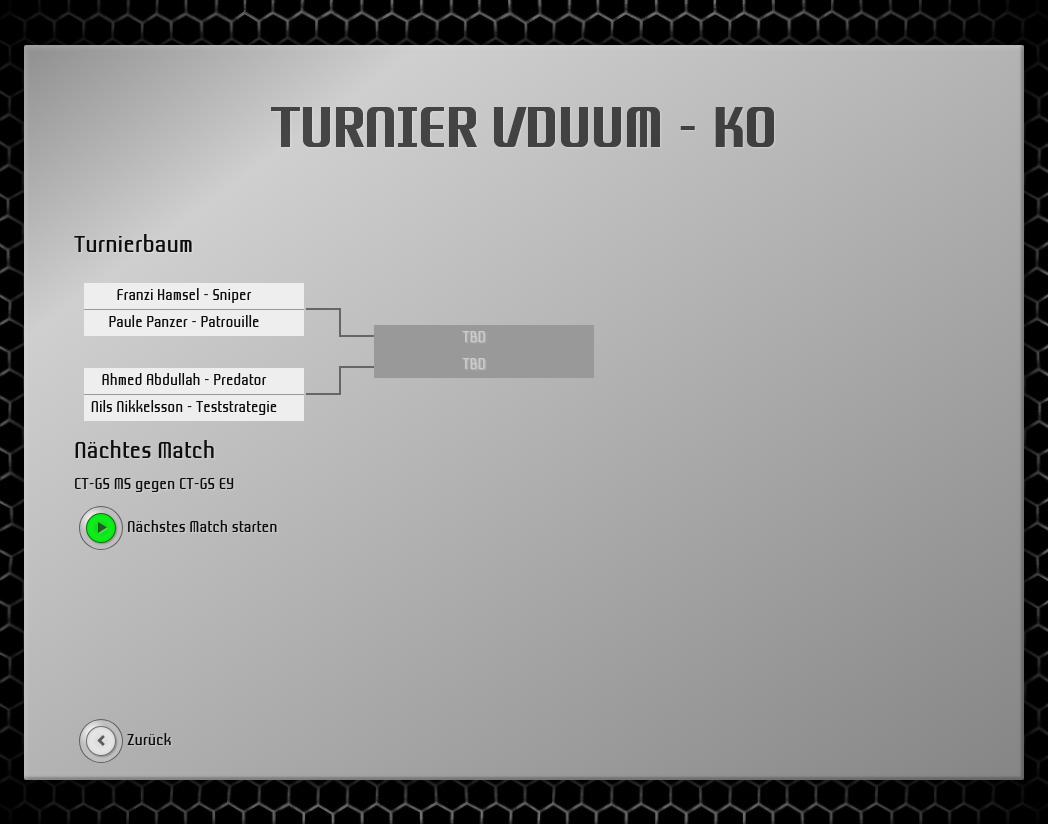
\includegraphics[width=15cm, keepaspectratio]{figures/16-turnierdurchfuehrung-ko-start.png}
  \caption{Die Übersicht zur Turnierdurchführung im KO-System bei Beginn des Turniers}
\end{figure}

\begin{figure}
  \centering
  \label{tournament-execution-ko-end}
  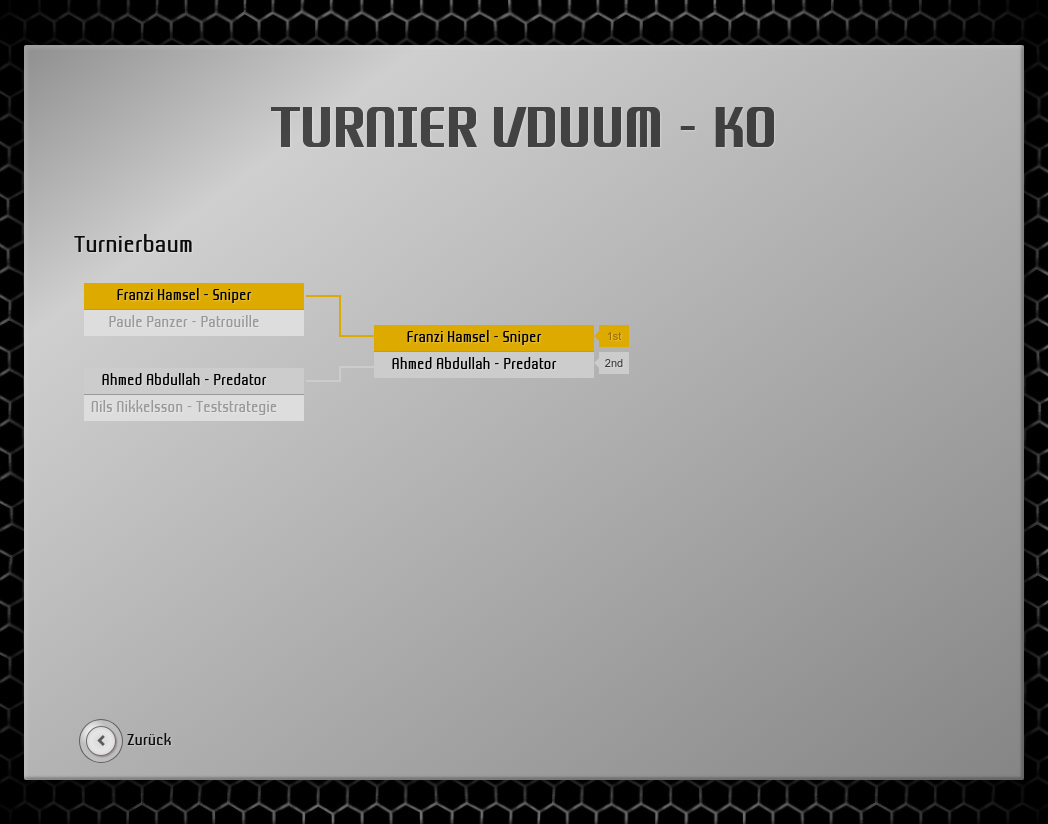
\includegraphics[width=15cm, keepaspectratio]{figures/16-turnierdurchfuehrung-ko-ende.png}
  \caption{Die Übersicht zur Turnierdurchführung im KO-System zum Ende des Turniers}
\end{figure}
